\section{Process' perspective}
\subsection{Developer interaction \& Team organization}
 In week 2 of the project we agreed on how we wanted to collaborate and described it in \href{https://raw.githubusercontent.com/Chillhound/DevOps2022F/main/CONTRIBUTE.md}{CONTRIBUTE.md}.

\subsubsection{Discord}
It was decided to use the communication platform \href{https://discord.com/}{\textit{Discord}}, which is great for facilitating discussions. The main communication line was in text channels. Voice channels were used to do collaboration sessions or further explain and share thoughts on the subjects from the text channels. During these online collaboration sessions we used screen sharing as a way to program in pairs.\\

\subsubsection{Physical meet-ups}
On Tuesdays after lecture, the developers would meet-up at the weekly exercise session and focus on the current weeks' workload. This was done so every team member could get insight in what was happening and could share thoughts and troubles that might occur during development of the project.

\subsection{Stages and tools in CI/CD chain}
\subsubsection{Tools}
A variety of different tools and technologies were used in the \textit{Continuous Integration} (CI) chain. 

The list below, summarizes tools and technologies used in the pipeline. 
\begin{itemize}
    \item Circle CI is a CI/CD service, and was used for the build server service.
    \item Docker Containers and Docker hub as a public artifact registry.
    \item SonarCloud used for static analysis.
    \item BetterCodeHub evaluates the GitHub code base against 10 software engineering guidelines.
    \item Digital Ocean a cloud server provider.
    \item GitHub Actions is used for building and linting the React project as well as compiling and generating a PDF report.
\end{itemize}

The configuration file for the CircleCI part of the pipeline is \href{https://raw.githubusercontent.com/Chillhound/DevOps2022F/main/.circleci/config.yml }{.circleci/config.yml} and the configuration files for GitHub actions are found in \href{https://github.com/Chillhound/DevOps2022F/tree/main/.github/workflows}{.github/workflows}.

\subsubsection*{Static analysis}
Included in the pipeline is also scanning of the frontend with SonarCloud and the backend with docker scan\footnote{\url{https://docs.docker.com/engine/scan/}}. \\
Moreover Better Code Hub\footnote{\url{https://bettercodehub.com/}} is used to scan the GitHub repository against 10 engineering guidelines devised by the authority in software quality, Software Improvement Group (SIG). 

\subsubsection{Stages}
The projects' CI/CD setup is implemented utilizing CircleCI and includes 3 primary stages: 
\begin{enumerate}
    \item Build docker image with frontend, scan the frontend, and push to Docker Hub.
    \item Build docker image backend, scan the image, and push to Docker Hub
    \item SSH into our DigitalOcean droplet to stop running containers, pull newest images from Docker Hub, curl the newest Docker Compose file and then start it all again with the Docker Compose file (\href{https://raw.githubusercontent.com/Chillhound/DevOps2022F/main/docker-compose-prod.yml}{docker-compose-prod.yml})
\end{enumerate}

The diagram in figure \ref{fig:CI} gives an overview of the CI pipeline and how we developers as well as the different platforms and technologies interact.
\begin{figure}[H]
 \centering
 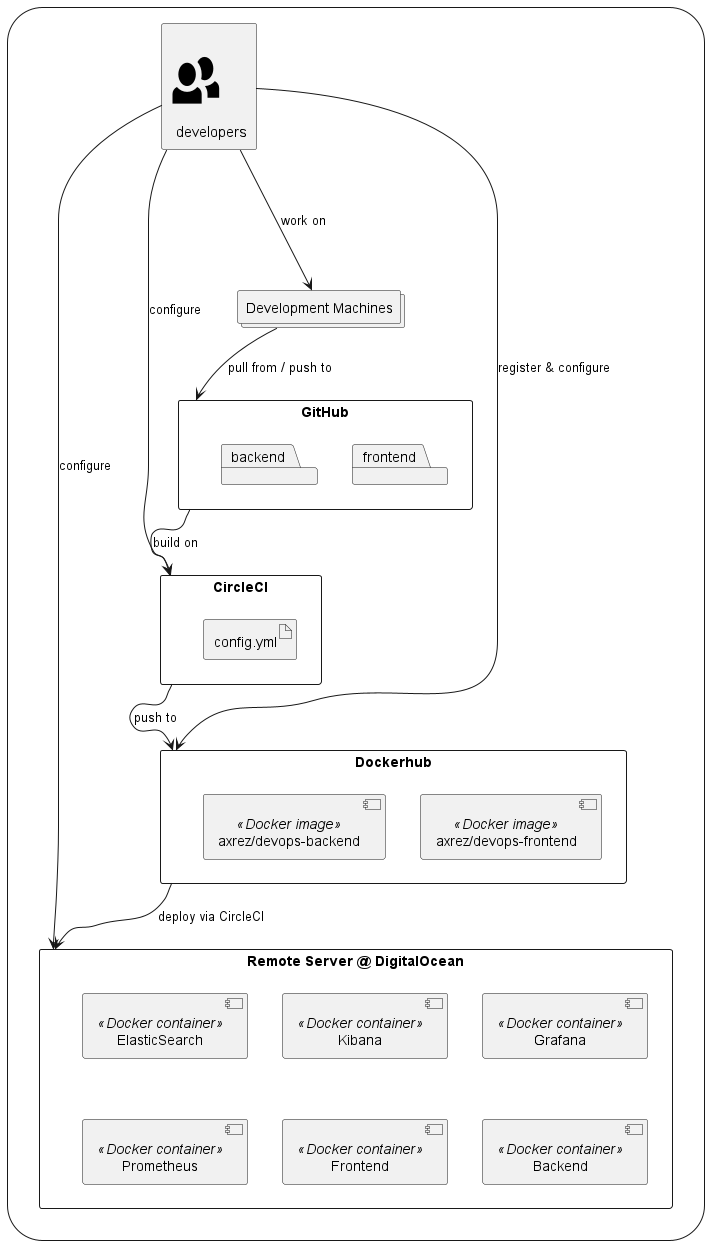
\includegraphics[width = .7 \textwidth]{images/ci.png}
 \caption{Overview of the CI pipeline}
 \label{fig:CI}
\end{figure}

\subsubsection{Environment variable}
The pipeline uses environment variables both in CircleCI and directly on our droplet to properly manage secrets like Docker Hub credentials, the database connection string and credentials for third party tools like Grafana, Elasticsearch and Kibana.

\subsubsection{Future plans}
At the moment, the CI/CD chain only deploys onto one droplet (primary) as seen in stage 3. Therefore, the project does not support for Continuous Deployment onto multiple droplets, this will have impact on an implementation with rolling updates, depending on the configuration. The thought was to deploy to a secondary droplet first and after that goes \textit{live}, redirect traffic from the primary droplet to the secondary. Shut-down the primary droplet and then deploy onto it, and after its live again redirect traffic back to the primary.

\subsection{Repository organization}
We have used a mono-repository setup for this project, where the root of the repository contains files related to configuration like Dockerfiles, Vagrantfiles etc. as well as two folders designated for frontend and backend code respectively.

\subsection{Applied branching strategy}
The branching strategy used is feature branching \cite{featurebranch}. The branches is organised in a main branch that contains the code base for the current running system. Main is also the target of our CI pipeline. \\
Feature branches are then branched out from main. When a feature is completed a pull request is opened, which needs to be reviewed and approved by a team member before it can get merged into main.

\subsection{Applied development process and tools supporting it}
During the project we have actively used GitHub issues to keep track of tasks both related to weekly assignments but also bugs, refactorings etc. that we have discovered or wanted to do ourselves. The issues is assigned labels to organize the priority, where the label \textit{important} is the most urgent and should be prioritised over a label like \textit{Nice-to-have}. To organise work on the issues the built-in Kanban board feature that GitHub provides is used during the development. This board helps the team with organizing the development, where the board shows what is being worked on by who. The board can be seen in Appendix \ref{app:githubboard}.   

\subsection{Monitoring}
%How do monitor and precisely what do you monitor? \\
To monitor the system the Prometheus package for .NET, \href{https://github.com/prometheus-net/prometheus-net}{\textit{prometheus-net}}, is used. Prometheus exposes some metrics from an ASP.net application by default. These metrics includes number of HTTP request in progress, number of received HTTP requests in total and duration of HTTP requests.
\\
A Grafana dashboard from the template: \href{https://grafana.com/grafana/dashboards/10915}{\textit{ASP.NET core - controller summary}} is used to visualize the technical monitoring information that Prometheus gathers from our system. The dashboard shows the following: \\
\noindent
\textbf{Business information}
\begin{itemize}
    \item Amount of users registered in the system
\end{itemize}
\textbf{Technical information}
\begin{itemize}
    \item Request received
    \item Error rate
    \item Total requests/s
    \item Request duration
    \item Number of requests in progress
\end{itemize}

Docker volumes are used to persist data from both Prometheus and Grafana.


The Grafana dashboard can be accessed at \href{http://157.245.27.14:3000/login}{http://157.245.27.14:3000/login} with the credentials provided during the course. \\
The raw monitoring metrics can be accesses through Prometheus at \href{http://157.245.27.14:9090/graph?g0.expr=&g0.tab=1&g0.stacked=0&g0.show_exemplars=0&g0.range_input=1h}{http://157.245.27.14:9090/}.


\subsection{Logging}
Our logging setup deviates from the popular ELK stack proposed in the \href{https://github.com/itu-devops/itu-minitwit-logging}{course material} and uses the following technologies. Instead of using Logstash the package Serilog is used in the system to aggregate logs.
\begin{itemize}
    \item Serilog\footnote{\url{https://serilog.net/}}
    \item ElasticSearch
    \item Kibana 
\end{itemize}
Serilog is imported as a dependency in the .NET project while both ElasticSearch and Kibana runs in their own respective Docker containers with volumes associated for persistence. The logs can have different log levels such as: debug, information, error, warning - which can be used for filtering.
The logging is centered around the simulator API and as such does not include e.g. the API used by the MiniTwit website.\\ 
The system logs can be accessed via Kibana at \href{http://157.245.27.14:5601/login?next=\%2F}{http://157.245.27.14:5601} with the credentials provided during the course.



\subsection{Security assessment}
Based on our security assessment we have taken precautionary steps which concretely has resulted in enabling DigitalOcean Two-Factor Authentication, enabling Dependabot and investigation of how we could add API Authentication. We have also talked about Security in relation to DDoS protection and developer-device security. The full Security assessment can be found in appendix \ref{app:SecurityAssessment}.

\subsection{Scaling and load balancing}
We chose to implement high-availability by using the configuration with Keepalived discussed in class, though with some modifications as the article\cite{KeepalivedUbuntu14} provided is deprecated. We have created our own updated version of Keepalived using Ubuntu 22 for documentation of the process and future use of others \footnote{\url{https://github.com/JacobMoller/Keepalived-DigitalOcean-Ubuntu-22.04/}}. \\
This means that we have two droplets on DigitalOcean - one which is our Primary droplet that we have had since the beginning of the project and one secondary which is activated if the primary crashes. A floating IP is used to support the setup.\\
The primary droplet contains all monitoring and logging and the secondary does not. \\
We agreed that, in case of an incident, the most important task is to be able to keep on serving clients, which is possible with this setup. We also agreed that the logs relevant to an incident e.g. before a crash, will come from the primary droplet and thus still be aggregated in this case.\\ If the secondary droplet goes active, we have an emergency situation that will need to be handled quickly and thus the lack of logging and monitoring is considered non-crucial. \\

Another approach to this would be to have a three droplet setup where monitoring and logging is located on the third droplet. This would allow the primary and secondary droplet to log to one central place. We chose not to do this as the third droplet would still be a single point of failure and because of what we agreed in regards to handling emergencies.\\

We have created alerts by email using sSMTP \footnote{\url{https://wiki.debian.org/sSMTP}} and Mailutils \footnote{\url{https://mailutils.org/}} which executes when the secondary droplet registers that the primary droplet is down (and therefore takes the floating IP). This allows us to be informed about this situation quickly and act upon it to recover and bring the service back to the primary droplet. \\
The email alerts are sent to all developers and can be seen in Appendix \ref{app:alert}.




